\subsection{Subsystem Testing}
% talks about different rigorous methods of testing the system

%\noindent FOV directivity test for range sensors, depression angle test, incoming data stream test.\\
% raise alerts if range threshold is crossed
% object detection test - range updates continuously and raises flag or interrupt if crosses below a threshold of danger
% - passing obstacle (confirm margin of safety)
% - moving obstacle
\subsubsection{Detection FOV Threshold} \label{ardumatlab}
\noindent The first test for the obstacle detection subsystem is straightforward. It will consist of the sensor readings code uploaded to the microcontroller, connected to a laptop which rests on the seat of the rollator. The serial plotter will be open and we aim to observe changes to pitch and yaw angles as well as sensor ranges all simultaneously. This will provide a visual indication and verification that the proper decisions based on detections can be created in the Senior Design II course. This test should work regardless of surface material and orientation of the obstacle. Therefore, it will be tested indoors in a hallway and open forum environment, outdoors in a neighborhood. The indoor test environments resemble that which FORWARD might be deployed in the medical hospital or assisted living facility, while it may also be driven around in lower calamity settings. Regardless, we will verify that ranging is independent of the environment.\\

\noindent Sensors must be integrated on the Medline rollator in their assigned positions, continuously transmitting the data to the microcontroller. The secondary goal will be to then connect the Arduino COM port to Matlab in order to generate a polar plot showcasing the field of vision of the rollator when outfitted with purely the range sensors. The three tiers of requirements for passing the test are as follows:
\begin{enumerate}
	\item \textbf{Basic:} Successfully detect face-on obstacles at $0.500$, $2.000$, $7.000$ meters. Range decreases and increases as the rollator is driven by the user.
	\item \textbf{Stretch:} Successfully detect obstacles at distance, at angles $\pm 15$, $\pm 30$, $\pm 90$ and sub-intervals depending on rollator attitude (degrees). Instantaneous delta in range measurement is observed when obstacle passes out of $S_x$ field of view
	\item \textbf{Advanced:} Alert the network "surrounded" or "hallway dead end" if all sensor ranges are below the 0.5 meter threshold.
\end{enumerate}
where a detection is defined by an instantaneous delta in the sensor readings, resulting in a less-than-maximum range. The distances are defined by radial distance from the center of mass of the rollator. The angles are defined in a polar manner, where the origin is also the center of mass. The coordinates $(x,y)$ of an obstacle $X_x$, detected by sensor $x$ at range $S_x$ and angle $\theta$ whose positive increase is counterclockwise in this frame is then given by:
$$X_x = S_x(cos(\theta), sin(\theta)) = (x,y)$$ \label{Polar}

\noindent As known, there are minor dead zones in the range sensors. Therefore, to determine a safe zone range threshold, it would need to exceed the range of dead sensing. Now, there could be a way to determine that FORWARD is reading the dead zone and coordinate emergency stops based on that (although it is also important to note that an emergency stop for low range may only be necessary if S2 and S3 front-facing are dead). The detection threshold can then be hard-coded into the GNC software, say $0.25$ meters.\\

\begin{figure}[H]
	\centering
	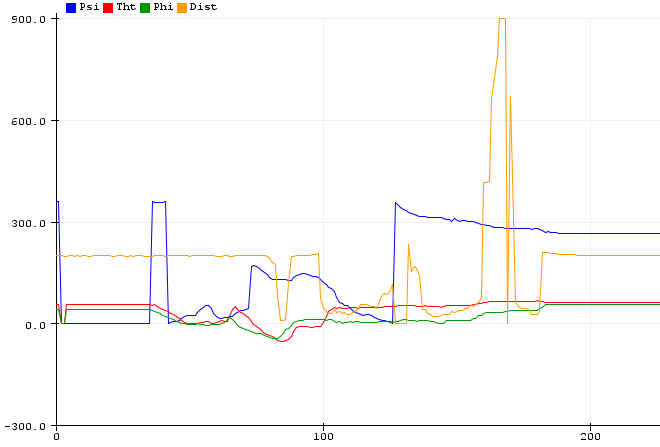
\includegraphics[width=0.7\textwidth]{./Images/serial-plotter.png}
	\caption{\label{fig:euler-test}Euler Angles Test}
\end{figure}

%\begin{figure}[H]
%	\centering
%	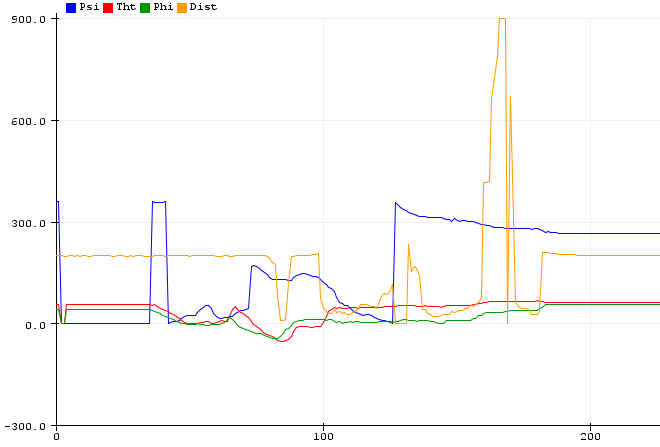
\includegraphics[width=0.7\textwidth]{./Images/serial-plotter.png}
%	\caption{\label{fig:range-test}Sensor Ranging Test}
%\end{figure}

\noindent It follows then, that we can define a range grid in polar coordinates where the maximum range detected is plotted versus yaw angle of the rollator. In this plot, we can also see precisely when there is an obstacle that causes a reduction in range.\\

% object identification test - classify obstacles and send walker into a moded resposne
% relay audio feedback to user informing them what is ahead
\subsubsection{Identification Importance}
\noindent It is crucial to assert an effective and accurate object identification system. To do this, we will implement a testing procedure to effectively test the goals outlined in this paper for FORWARD. The test for the basic goals will be to provide the camera with each of the objects listed to be identified, using 10 different versions of each at varied locations in the camera FOV. We will run this test 10 times each to obtain a percentage pass/fail for the necessary objects. For the stretch goals, we will provide the camera with a few different environments of similar danger, i.e. different crowded environments, different parking lots, etc. and record the percentage of passing tests, looking to achieve a confidence level of at least 80\% before including this technology in FORWARD. For our Advanced goals, we will test this by moving FORWARD towards a grassy field or wall and recording the point in which the system determines a static obstacle. We will then adjust the scale for classifying such obstacles until we identify these obstacle types with at least 3 feet of clearance. \\

The tiers of testing goals are:
\begin{enumerate}
	\item \textbf{Basic:} Alert the network there is a certain type of obstacle present (i.e. person, dog, car).
	\item \textbf{Stretch:} Alert the network that if two or more cars are present, "road ahead." If two or more people are present, "crowd ahead." Rank how urgent the situation is.
	\item \textbf{Advanced:} If range sensors return low but no obstacles classified, alert the network "wall." This is a placeholder code for any static solid obstacle.
\end{enumerate}

% object avoidance test - activate feedback and update motor speeds
\subsubsection{Control Feedback}
\noindent We must likewise test the haptic motors to determine if they are operational. The most important goal for this evaluation is to ensure that the components purchased are not defective, the wiring is correct, and that the programming also is correct. There are a number of issues that could arise within these processes, so simply spinning the motors would be a victory for this test. However, we will be more prepared for Senior Design II if we are able to incorporate the programming controlling the haptic motors with the rest of the code. This would involve the motors altering their vibration as a result of the sensor data and/or identifying the location of the obstacle as either on the left or right. We will zip tie the motors to the handlebars and then test the haptic feedback in a similar way as we will test the sensors. The rollator will be walked down a hallway and turned to face the wall, thus providing a difference in sensor readings. Ideally, the motors will vibrate in response to a change in distance from the ultrasonic sensors. A successful control feedback test is defined by:

\begin{enumerate}
	\item \textbf{Basic:} Successfully vibrate the rollator handlebars via the haptic motors attached.
	\item \textbf{Stretch:} Increase the frequency of vibration as range reading decreases.
	\item \textbf{Advanced:} Spatially aware haptic feedback - left and right handlebars indicate the location of the obstacle.
\end{enumerate}

 
 \noindent In addition to vibration, we will include serial print statements within the software so that we can easily troubleshoot incorrect behavior from the haptics. If the statement printed in serial is not corresponding to the actions of the motors, we know that there is a hardware issue, either with the MCU, motors, or wiring. Contrarily, if the expected statement is not printed in the serial monitor, we can reasonably assume that there is a software issue.\\

% in SD2, will need to refine turning ratios, hazard range thresholds, and work on stretch requirements.
\subsection{System Integration, Testing, and Evaluation}
\noindent System integration was already incorporated to some extent into the subsystem testing described in the previous subsection. However, there will be further concerns and scrutiny the FORWARD system must be subjected to as a whole. Among basic properties such as secure mounting and housing in the electronics chassis (discussed in section \ref{chassis}), it is good to consider waterproofing, temperature, viability with low battery/power supply, and configurations with sensors on, camera off, or vice versa. This should be done in order to ensure a reliable product is brought to the user.\\

\noindent \underline{\textit{PCB Assembly and Testing}}
\noindent As mentioned, the printed circuit board should be tested with varying levels of battery life remaining. It is likely that we will need to order a new PCB after testing our initial PCB as it is common for there to be issues such as changes in components, missed voltage regulation requirements, broken connections, incorrect sizing, lack of electrical isolation, or miswiring. Of course we will attempt to prepare for these mishaps, yet there is still a necessity  for testing and evaluation.\\

\noindent \underline{\textit{Determining and tuning motor coefficients}} During integration, it will be necessary to assign values governing the yaw steering command to the speed of the motors and haptic feedback signals. There should exist some constants that taking into account the rollator dynamics, can be calculated to scale the motors in order to achieve the desired turning angle. Additionally, once integration has been achieved, these scalars can be fine-tuned to optimize the rollator performance response.\\

\noindent \underline{\textit{Autonomous Navigation with Cooperative User}}
\noindent With motors installed on the rollator, which is also equipped with GNC software, there should be decision-making in the main code to distinguish how FORWARD adapts based on the environment. Some scenarios that come to mind are:
\begin{enumerate}
	\item Evasive mode. FORWARD takes full control (i.e. emergency stop)
	\item Cooperative navigation mode. FORWARD guides the user in a way does not infringe on their free movement.
	\item Dormant mode. User has full control of direction. \footnote{This is distinct from system powered off because the electronics are still in operation, they are just not being stimulated from the environment in a way that demands response from FORWARD}
\end{enumerate}
This step is probably the most difficult to implement at the same time as PCB development, motor coefficient tuning, and critical design review are taking place. Oftentimes, system moding is not as straightforward as it is cut out to be; in the boundary conditions when FORWARD will transition from one mode to the next, the team will have to carefully design the GNC software to remain stable. In other words, it remains subjective exactly when to apply emergency braking or how to define edge cases of multi-obstacle scenarios. Curb lifting, headlights in lowlight environments, and the other advanced requirements also remain undefined at this time.\\

\noindent \underline{\textit{Free Roam Evaluation}}
\noindent The final phase of testing is done when FORWARD integration is complete, and this is called the free roam evaluation. Essentially, the walker will be driven out in public for a pre-determined period of time, and the team will note mishaps and incidents that the guidance, navigation, and control protocols fail to prevent. These would be noted for future improvements for future endeavors and projects or products. This evaluation method will truly test and determine the successful or unsuccessful implementation of FORWARD from the beginning specifications and requirements listed. Multi-obstacle scenarios, mixtures of incline and decline territories, and mild levels of danger will be encountered. If requirements are met, design is up to specification, and all previous tests have been passed, we are confident FORWARD evaluation will be a success.\\

\subsection{Evaluation of Test Results}
\noindent We have successfully been able to test at least one major component from each subsystem. Minimally, the basic goals for each of these subsystems has been met, and some subsystems were even able to achieve the stretch goals for testing.\\

\subsubsection{Sensor Evaluation}
\noindent We have accomplished the stretch goals for this subsystem. This entails not only detecting obstacles at particular range, but also rotating the walker to measure the angle of rotation and ensure proper detection of obstacles. We exceeded these requirements in that all three sensors were taking measurements. However, we did not add a case for the serial monitor to determine if the sensor ranges indicate "surrounded" or "hallway dead end."\\

\noindent \underline{\textit{IMU Testing}} \noindent The first sensor that we verified operates as intended was the IMU. This involved testing the three angles of pitch, yaw, and roll. The IMU was mounted on the chassis of the rollator, so when we rotated the walker in a circle, the yaw angle incresaed linearly until the rollator had rotate 360 degrees and was rest to zero degrees. The pitch of the IMU was verified by applying pressure to the handlebars so that the front wheels were elevated, thus tilting the rollator upward and causing the angle to increase. The final angle, roll, of the walker was tried by applying pressure to one side of the walker so that the other side was elevated above the ground. This causes the roll angle to increase. The IMU also has the capabilities to measure the acceleration in the x, y, and z directions. We noted that as we started running with the walker, the acceleration increased in the x direction.\\

\noindent \underline{\textit{Ultrasonic Testing}}
\noindent The testing for the ultrasonic sensors was quite simple. We mounted two sensors to the front of the chassis and two on either side of the chassis. Testing in the midst of a long hallway, the ultrasonics at first could not read any obstacles in front of the walker as it faced the length of the hallway. Then as someone stepped in front of the walker, the distance measured from the ultrasonics decreased. Steering the rollator to be near the wall, the distance also decreased, and as we drove along the wall, the ultrasonic sensors to the side of the rollator decreased in distance.\\

\noindent \underline{\textit{LiDAR Testing}} \noindent The LiDAR sensor was mounted in the center of the chassis facing straight ahead. It was able to detect when an object was directly in front of the walker. When one of our team members waved his hand in front of the LiDAR, the Euler Angles Test reflected this change in distance by fluctuating values in spikes. While there exists no object in the path straight ahead of the walker, the LiDAR reads either reads a high value (large distance between sensor and object) or a value of zero, meaning the object is so far that the maximum range is exceeded. When an object was in view, the reading of the LiDAR fluctuates to reflect the range either decreasing from a large range or increasing from zero.\\

\subsubsection{Camera Evaluation}
\noindent The object identification subsystem underwent evaluation as well. For this evaluation, we simply met the basic goals of testing in which objects in the field of view are identified. The camera module was attached to the center of the rollator chassis objects, including a person, a chair, and a photo of a dog, were placed in front of the camera. The MCU used this module to capture both the identify of the obstacle and its location within the window frame. The MCU correctly processed the camera input to classify each obstacle as a person, a chair, and a dog, respectively, and the results were displayed in the serial monitor.\\

\subsubsection{Haptic Evaluation}
\noindent Within our system testing, we have accomplished more than the basic goal for operating the haptic feedback motors. The motors were able to vibrate as a result of our MCU programming and have been integrated to depend on sensor readings. When attached to the frame of the rollator, the handlebars successfully reverberated.\\

\noindent Although our initial stretch goal was to increase the frequency of vibration as the sensor range reading decreased, we were unable to properly test this functionality. Our current theory as to why we could not tell the difference between the haptic motor vibration intensity as range decreased is that the haptic motors do not vary much in duty cycle. This is because we needed a duty cycle of around 150 before the motors seemed to noticeably vibrate. Thus, the duty cycles used to vibrate within different ranges were 150, 200, and 255. We were unable to detect a difference as we changed the duty cycle as a result of the ultrasonic readings, however, it was not clear to us if there was a programming issue or if the PWM cycles are simply too close together to notice a difference.\\

\noindent We still consider testing for the haptic motors more than successful because integration was made possible between the haptics and the ultrasonic sensors. The haptic code was synthesized with the main code that controlled both the camera and sensor input. Not only was one of the motors able to vibrate while the sensors were operational, they gave feedback when obstacles were detected to the left or in front of the walker. When the ultrasonic reading was less than around 1-2 feet, then the motor would vibrate.\\

\noindent We were unable to achieve the advanced goal of spatially aware feedback due to an unknown issue in wiring. At the outset of our testing, both haptic motors were functioning properly and vibrating in sequence. During the same program, the right haptic motor ceased vibrating despite our efforts to check connections and ensure we were operating from the same code. After probing with the digital multimeter, we discovered that voltage was no longer being applied to the Output 2 terminals of the motor driver. Further testing will be required to troubleshoot the issue.\\